\documentclass{beamer}

\newcommand{\course}{CS 1331 Introduction to Object Oriented Programming}
\newcommand{\lesson}{Swing, Part 2 of 5}
\newcommand{\code}{http://www.cc.gatech.edu/~simpkins/teaching/gatech/cs1331/code}

\author[Chris Simpkins] 
{Christopher Simpkins \\\texttt{chris.simpkins@gatech.edu}}
\institute[Georgia Tech] % (optional, but mostly needed)

\date[CS 1331]{}

\subject{\lesson}


% If you have a file called "university-logo-filename.xxx", where xxx
% is a graphic format that can be processed by latex or pdflatex,
% resp., then you can add a logo as follows:

% \pgfdeclareimage[width=0.6in]{coc-logo}{cc_2012_logo}
% \logo{\pgfuseimage{coc-logo}}

\mode<presentation>
{
  \usetheme{Berlin}
  \useoutertheme{infolines}

  % or ...

 \setbeamercovered{transparent}
  % or whatever (possibly just delete it)
}

\usepackage{hyperref}
\usepackage{fancybox}
\usepackage{listings}
\usepackage[abbr]{harvard}

\usepackage[english]{babel}
% or whatever

\usepackage[utf8]{inputenc}
% or whatever

\usepackage{times}
\usepackage[T1]{fontenc}
% Or whatever. Note that the encoding and the font should match. If T1
% does not look nice, try deleting the line with the fontenc.


\usepackage{listings}
 
% "define" Scala
\lstdefinelanguage{scala}{
  morekeywords={abstract,case,catch,class,def,%
    do,else,extends,false,final,finally,%
    for,if,implicit,import,match,mixin,%
    new,null,object,override,package,%
    private,protected,requires,return,sealed,%
    super,this,throw,trait,true,try,%
    type,val,var,while,with,yield},
  otherkeywords={=>,<-,<\%,<:,>:,\#,@},
  sensitive=true,
  morecomment=[l]{//},
  morecomment=[n]{/*}{*/},
  morestring=[b]",
  morestring=[b]',
  morestring=[b]""",
}

\usepackage{color}
\definecolor{dkgreen}{rgb}{0,0.6,0}
\definecolor{gray}{rgb}{0.5,0.5,0.5}
\definecolor{mauve}{rgb}{0.58,0,0.82}
 
% Default settings for code listings
\lstset{frame=tb,
  language=scala,
  aboveskip=2mm,
  belowskip=2mm,
  showstringspaces=false,
  columns=flexible,
  basicstyle={\scriptsize\ttfamily},
  numbers=none,
  numberstyle=\tiny\color{gray},
  keywordstyle=\color{blue},
  commentstyle=\color{dkgreen},
  stringstyle=\color{mauve},
  frame=single,
  breaklines=true,
  breakatwhitespace=true,
  keepspaces=true
  %tabsize=3
}


\title[\course] % (optional, use only with long
                                      % paper titles)
{\lesson}

\subtitle{}
%% {Include Only If Paper Has a Subtitle}

\newcommand{\link}[2]{\href{#1}{\textcolor{blue}{\underline{#2}}}}


% If you wish to uncover everything in a step-wise fashion, uncomment
% the following command: 

% \beamerdefaultoverlayspecification{<+->}


\begin{document}

\begin{frame}
  \titlepage
\end{frame}

%------------------------------------------------------------------------
\begin{frame}[fragile]{Outline}


\begin{itemize}
\item Components and Containers
\item Layout Managers
\item Listening to multiple components
\item Menus
\end{itemize}


\end{frame}
%------------------------------------------------------------------------

%------------------------------------------------------------------------
\begin{frame}[fragile]{Components and Containers}


\begin{itemize}
\item A component is an object with a visual representation in the GUI.
\item A container is a component that contains other componets.
\item Most GUI aplications have multiple components, and thus need containers to manage them.
\end{itemize}
For example, this CounterFrame has four {\tt java.awt.Component}s:
\begin{columns}[c]
\begin{column}{2in}
\begin{center}
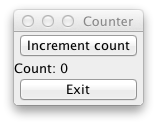
\includegraphics[width=1.75in]{CounterFrame.png}
\end{center}
\end{column}
\begin{column}{3in}
\begin{itemize}
\item a {\tt javax.swing.JButton} labeled ``Increment count'',
\item a {\tt javax.swing.JLabel} that displays the count,
\item a {\tt javax.swing.JButton} labeled ``Exit'', and
\item a {\tt javax.swing.JFrame} that contains the other three components.
\end{itemize}
\end{column}
\end{columns}

\end{frame}
%------------------------------------------------------------------------

%------------------------------------------------------------------------
\begin{frame}[fragile]{Layout Managers}

\begin{itemize}
\item Layout managers control the position of components in a container.
\item {\tt CounterFrame} uses a {\tt java.awt.BorderLayout}.
\item {\tt java.awt.BorderLayout} places components in one of 5 regions:
\end{itemize}
\vspace{-.05in}
\begin{center}
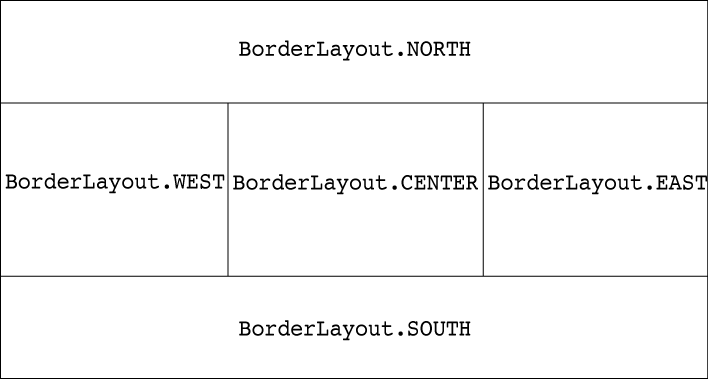
\includegraphics[height=2in]{border-layout.png}
\end{center}


\end{frame}
%------------------------------------------------------------------------

%------------------------------------------------------------------------
\begin{frame}[fragile]{Using a BorderLayout}


To use a BorderLayout, import {\tt java.awt.BorderLayout}:

\begin{lstlisting}[language=Java]
import java.awt.BorderLayout;
\end{lstlisting}

Call the {\tt setLayout} method in {\tt java.awt.Container} (here {\tt CounterFrame} is a subclass of {\tt JFrame}, which is a subclass of {\tt java.awt.Container})\footnote{Technically, {\tt JFrame} contains a {\tt JRootPane} container for all non-menu components, which is returned by {\tt JFrame}'s {\tt getContentPane} method.  For convenience, {\tt JFrame}'s {\tt setLayout}, {\tt add}, and {\tt remove} methods forward to the content pane.}
\begin{lstlisting}[language=Java]
setLayout(new BorderLayout());
\end{lstlisting}

See \link{\code/swing/CounterFrame.java}{CounterFrame.java} for the full code referenced above.

\end{frame}
%------------------------------------------------------------------------

%------------------------------------------------------------------------
\begin{frame}[fragile]{Adding Components Using a Layout Manager}


When you add a component to a container, you often pass layout manager-specific arguments to the {\tt add} method to specify where the component should go.  For example, using a {\tt BorderLayout} in {\tt CounterFrame}'s constructor:
\begin{lstlisting}[language=Java]
add(counterButton, BorderLayout.NORTH);
add(counterLabel, BorderLayout.CENTER);
add(exitButton, BorderLayout.SOUTH);
\end{lstlisting}
To use a {\tt GridLayout}, simply add components in row-major order:
\begin{lstlisting}[language=Java]
setLayout(new GridLayout(3,1)); // 3 rows, 1 column
add(counterButton);
add(counterLabel);
add(exitButton);
\end{lstlisting}

Becoming proficient at laying out GUI components requires practice.  Have a look at \link{http://docs.oracle.com/javase/tutorial/uiswing/layout/index.html}{Oracle's tutorial} and experiment with the sample code we provide.

\end{frame}
%------------------------------------------------------------------------

%------------------------------------------------------------------------
\begin{frame}[fragile]{Nesting Containers}


Containers can be nested for more complex layouts:
\begin{center}
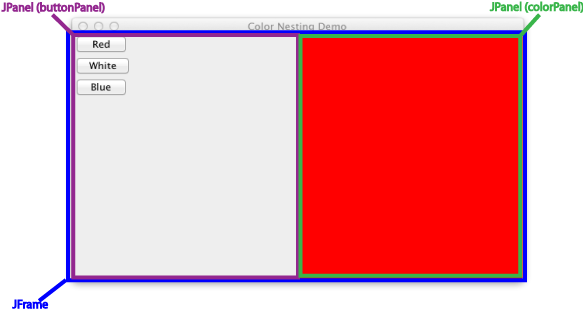
\includegraphics[width=4.5in]{nesting-containers.png}
\end{center}


\end{frame}
%------------------------------------------------------------------------

%------------------------------------------------------------------------
\begin{frame}[fragile]{Creating Nested Containers}
\vspace{-.05in}
\begin{itemize}
\item Create components from inside out: first UI widgets, then their inner containers, then outer container(s):
\end{itemize}
\vspace{-.1in}
\begin{lstlisting}[language=Java]
// Set up button panel
JButton redButton = new JButton("Red");
redButton.addActionListener(this);
// ...
JPanel buttonPanel = new JPanel();
buttonPanel.setLayout(new BoxLayout(buttonPanel, BoxLayout.Y_AXIS));    
buttonPanel.add(redButton);
// ...
// Set up color panel
colorPanel = new JPanel();
colorPanel.setSize(200, 200);
// Set up main application frame
setDefaultCloseOperation(JFrame.EXIT_ON_CLOSE);
setLayout(new GridLayout(1, 1)); // 1 row, 1 column
add(buttonPanel);
add(colorPanel);
\end{lstlisting}
\vspace{-.05in}
See \link{\code/swing/ColorBox.java}{ColorBox.java} for full code.
\end{frame}
%------------------------------------------------------------------------

%------------------------------------------------------------------------
\begin{frame}[fragile]{Listening to Multiple Components}

\vspace{-.05in}
Notice that \link{\code/swing/ColorBox.java}{ColorBox.java} implements {\tt ActionListener}:
\vspace{-.05in}
\begin{lstlisting}[language=Java]
public class ColorBox extends JFrame implements ActionListener { ...
\end{lstlisting}
We register the {\tt ColorBox} instance as a listener to its own components using {\tt this}:
\vspace{-.1in}
\begin{lstlisting}[language=Java]
redButton.addActionListener(this);
\end{lstlisting}
And implement the {\tt actionPerformed} method:
\vspace{-.1in}
\begin{lstlisting}[language=Java]
public void actionPerformed(ActionEvent e) {
    String button = e.getActionCommand();
    if (button == "Red") {
        colorPanel.setBackground(Color.RED);
    } else if ...
\end{lstlisting}
\vspace{-.1in}
\begin{itemize}
\item Each component has an {\tt actionCommand} that's passsed into its constructor or set with {\tt setActionCommand(String s)}.
\item You can use the {\tt actionCommand} to identify which component fired an event.
\end{itemize}


\end{frame}
%------------------------------------------------------------------------

%------------------------------------------------------------------------
\begin{frame}[fragile]{Adding Menus}

\vspace{-.05in}
\begin{itemize}
\item Create {\tt JMenuItem}s, add listeners to them.
\item Create {\tt JMenu}s, add {\tt JMenuItem}s to them.
\item Create a {\tt JMenuBar}, add {\tt JMenu}s to it.
\item Set the {\tt JMenuBar} as the frame's menu
\end{itemize}
The entire process for a simple 3-item color menu is:
\vspace{-.05in}
\begin{lstlisting}[language=Java]
JMenuItem redMenuItem = new JMenuItem("Red");
redMenuItem.addActionListener(this);
/ ...
JMenu colorMenu = new JMenu("Color");
colorMenu.add(redMenuItem);
// ...
JMenuBar menuBar = new JMenuBar();
menuBar.add(colorMenu);
setJMenuBar(menuBar);
\end{lstlisting}
\vspace{-.1in}
\begin{itemize}
\item Notice that you add action listeners to {\tt JMenuItem}s the same way you add them to {\tt JButton}s.
\item {\tt javax.swing.JMenuItem} and {\tt javax.swing.JButton} are both subclasses of {\tt javax.swing.AbstractButton}.  
\end{itemize}
\end{frame}
%------------------------------------------------------------------------

%------------------------------------------------------------------------
\begin{frame}[fragile]{Closing Thoughts}


\begin{itemize}
\item GUI programming requires two things:
\begin{itemize}
  \item Knowledge of GUIs (widgets, how they work, how they're used)
  \item Knowledge of a particular GUI framework (like Swing)
\end{itemize}
\item The Swing classes you've seen make extensive use of OOP (like {\tt JMenuItem} and {\tt JButton} being subclasses of {\tt AbstractButton}.
\item GUI programs are straightforward, but get complex quickly.
\item In the next few lectures, we'll begin to learn how to deal with the complexity of GUI programs with the Model-View-Controller pattern.
\end{itemize}


\end{frame}
%------------------------------------------------------------------------




% %------------------------------------------------------------------------
% \begin{frame}[fragile]{}


% \begin{lstlisting}[language=Java]

% \end{lstlisting}

% \begin{itemize}
% \item
% \end{itemize}


% \end{frame}
% %------------------------------------------------------------------------


\end{document}
